\documentclass{article}
\usepackage[school,simplified]{pgf-umlcd}
\usepackage[margin=2.5cm]{geometry}
\usepackage[utf8]{inputenc}
\usepackage[T1]{fontenc} % ensure that all the characters in characterSets.tex prints

\begin{document}
\section*{Classes}
\begin{center}
  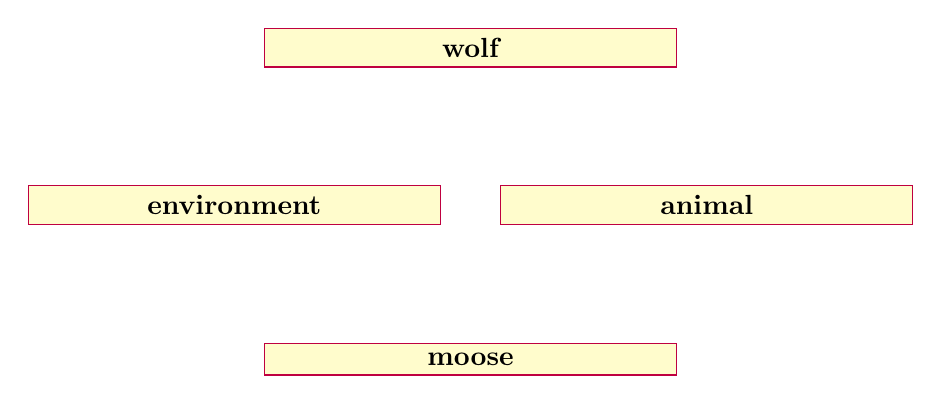
\begin{tikzpicture}
    \begin{class}[text width=5cm]{animal}{0,0}
    \end{class}
    \begin{class}[text width=5cm]{moose}{-3,-2}
    \end{class}
    \begin{class}[text width=5cm]{wolf}{-3,2}
    \end{class}
    \begin{class}[text width=5cm]{environment}{-6,0}
    \end{class}
  \end{tikzpicture}
\end{center}

\section*{Inheritance}
\begin{center}
  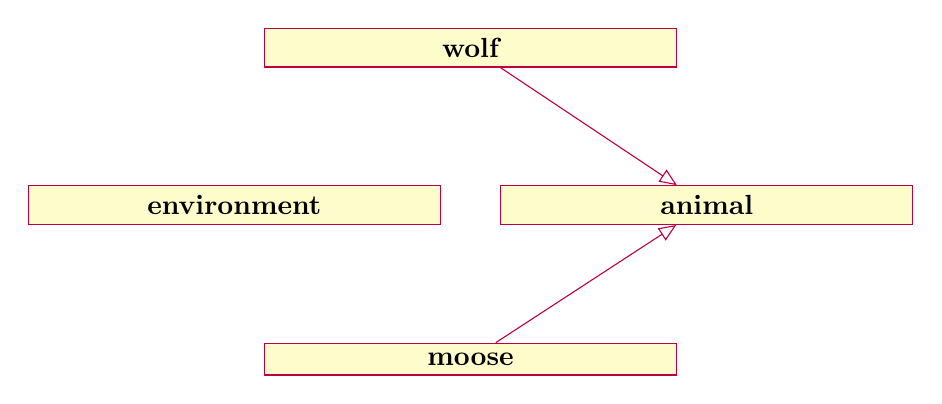
\begin{tikzpicture}
    \begin{class}[text width=5cm]{animal}{0,0}
    \end{class}
    \begin{class}[text width=5cm]{moose}{-3,-2}
      \inherit{animal}
    \end{class}
    \begin{class}[text width=5cm]{wolf}{-3,2}
      \inherit{animal}
    \end{class}
    \begin{class}[text width=5cm]{environment}{-6,0}
    \end{class}
  \end{tikzpicture}
\end{center}
\vspace*{1cm}

\begin{center}
  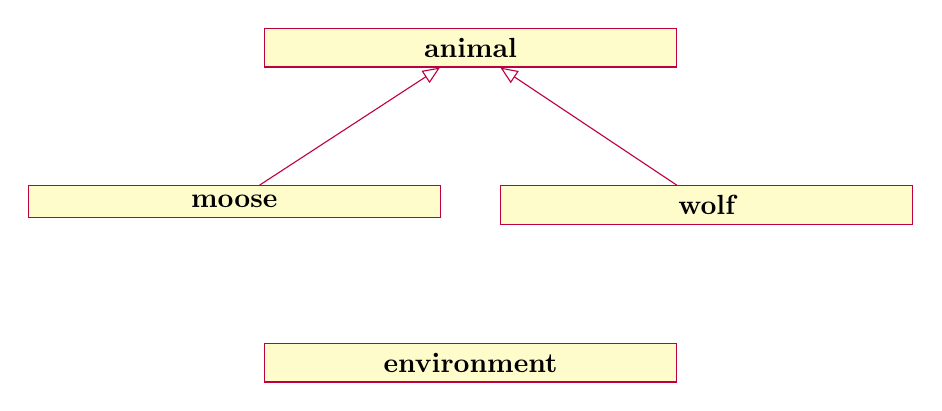
\begin{tikzpicture}
    \begin{class}[text width=5cm]{animal}{0,0}
    \end{class}
    \begin{class}[text width=5cm]{moose}{-3,-2}
      \inherit{animal}
    \end{class}
    \begin{class}[text width=5cm]{wolf}{3,-2}
      \inherit{animal}
    \end{class}
    \begin{class}[text width=5cm]{environment}{0,-4}
    \end{class}
  \end{tikzpicture}
\end{center}

\section*{Associations}
\begin{description}
\item[Association]~\\
  Host 'kender til' gæst
\item[Aggregation]~\\
  Host 'har kopi af' gæst
\item[Composition]~\\
  Host 'opretter afhængig og har kopi af' gæst. Når host slettes slettes gæst ligeså.
\end{description}

\begin{center}
  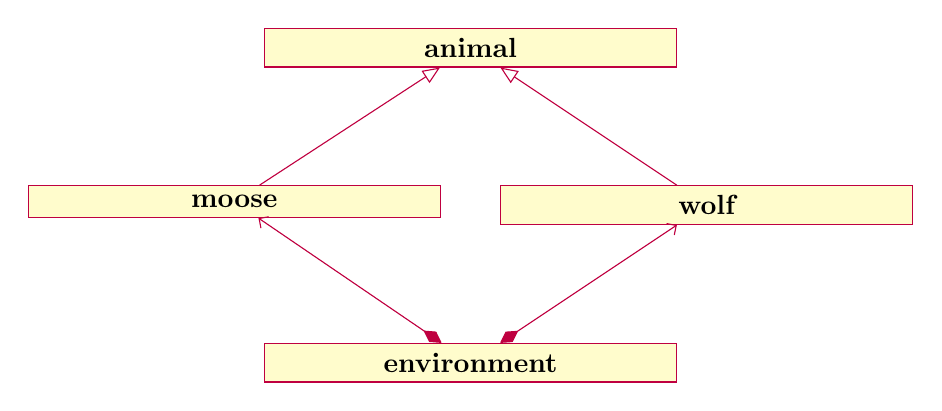
\begin{tikzpicture}
    \begin{class}[text width=5cm]{animal}{0,0}
    \end{class}
    \begin{class}[text width=5cm]{moose}{-3,-2}
      \inherit{animal}
    \end{class}
    \begin{class}[text width=5cm]{wolf}{3,-2}
      \inherit{animal}
    \end{class}
    \begin{class}[text width=5cm]{environment}{0,-4}
    \end{class}
    \composition{environment}{}{}{moose}
    \composition{environment}{}{}{wolf}
  \end{tikzpicture}
\end{center}


\section*{Relations}
\begin{center}
  \fbox{
    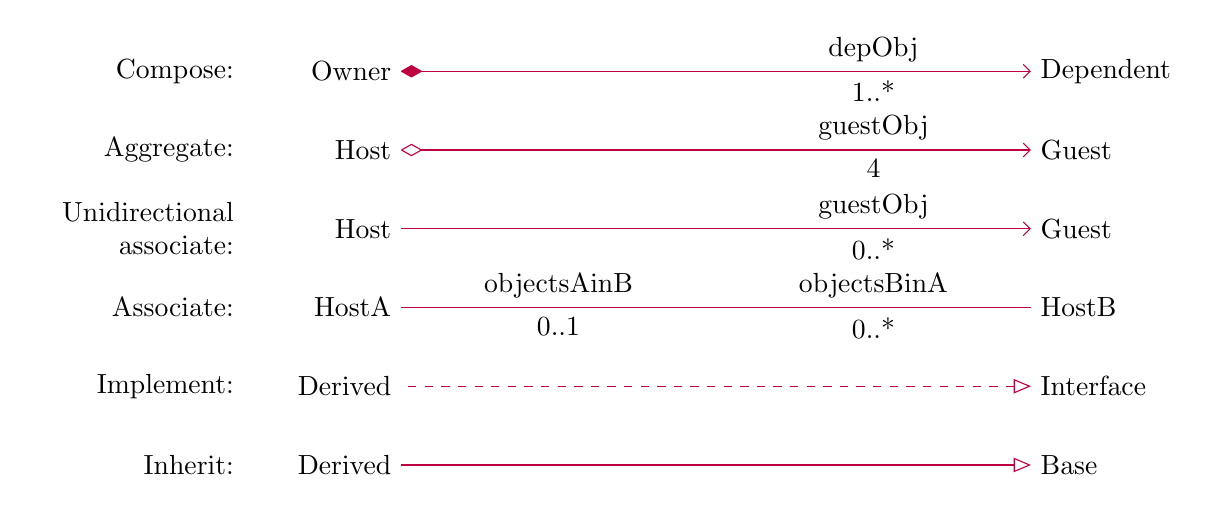
\begin{tikzpicture}
      % \draw[umlcd style dashed line] (0,4) --(8,4);
      % \draw[splitline] (0,3) --(8,3);
      \node [left] at (-2,5) {Compose:}; \node (composeLeft) [left] at
      (0,5) {Owner}; \node (composeRight) [right] at (8,5)
      {Dependent};
      \composition{composeLeft}{depObj}{1..*}{composeRight};
      
      \node [left] at (-2,4) {Aggregate:}; \node (aggregateLeft)
      [left] at (0,4) {Host}; \node (aggregateRight) [right] at (8,4)
      {Guest};
      \aggregation{aggregateLeft}{guestObj}{4}{aggregateRight};
      
      \node [left] at (-2,3) {\parbox[r]{2.5cm}{\raggedleft
          Unidirectional associate:}}; \node (uniAssociateLeft) [left]
      at (0,3) {Host}; \node (uniAssociateRight) [right] at (8,3)
      {Guest};
      \unidirectionalAssociation{uniAssociateLeft}{guestObj}{0..*}{uniAssociateRight};

      \node [left] at (-2,2) {Associate:}; \node (associateLeft)
      [left] at (0,2) {HostA}; \node (associateRight) [right] at (8,2)
      {HostB};
      \association{associateLeft}{objectsAinB}{0..1}{associateRight}{objectsBinA}{0..*}
      ;
      
      \node [left] at (-2,1) {Implement:}; \node (interfaceDerived)
      [left] at (0,1) {Derived}; \node (interfaceBase) [right] at
      (8,1) {Interface}; \draw[umlcd style implement line]
      (interfaceBase) -- (interfaceDerived);
      
      \node [left] at (-2,0) {Inherit:}; \node (inheritDerived) [left]
      at (0,0) {Derived}; \node (inheritBase) [right] at (8,0) {Base};
      \draw[umlcd style inherit line] (inheritBase) --
      (inheritDerived);
    \end{tikzpicture}
  }
\end{center}

\section*{Properties and methods}
\begin{center}
  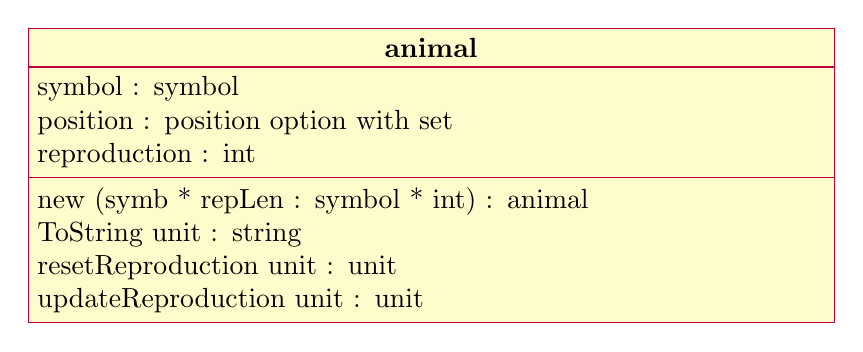
\begin{tikzpicture}
    \begin{class}[text width=10cm]{animal}{0,0}
      \attribute{symbol : symbol}
      \attribute{position : position option with set}
      \attribute{reproduction : int}
      \operation{new (symb * repLen : symbol * int) : animal}
      \operation{ToString  unit : string}
      \operation{resetReproduction  unit : unit}
      \operation{updateReproduction  unit : unit}
    \end{class}
  \end{tikzpicture}
\end{center}
\vspace*{1cm}

\begin{center}
  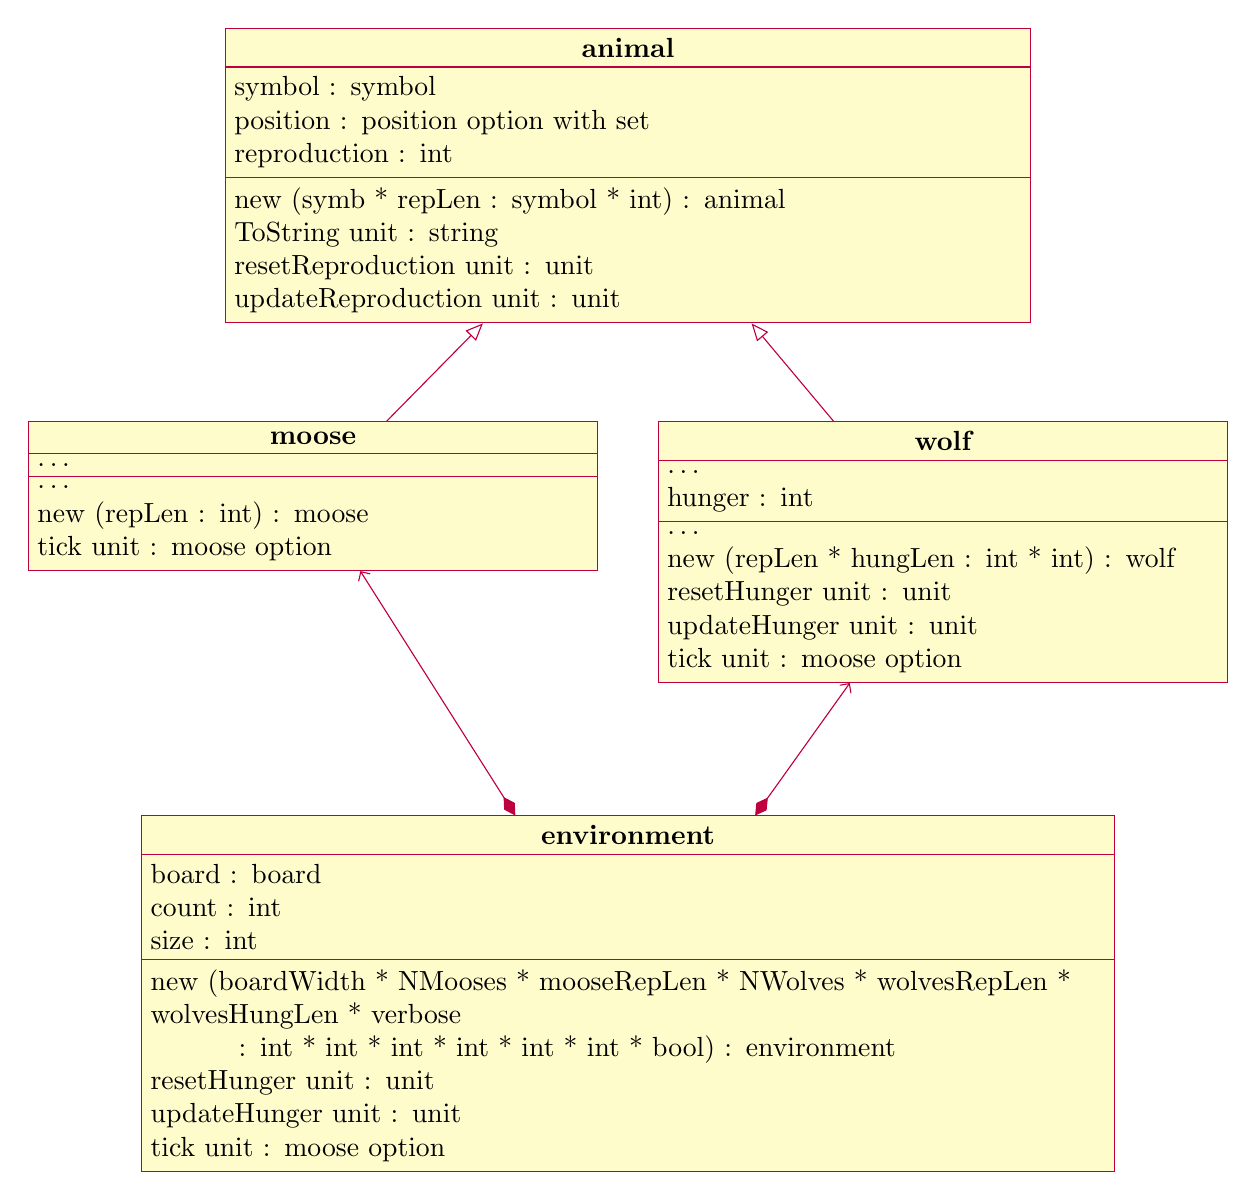
\begin{tikzpicture}
    \begin{class}[text width=10cm]{animal}{0,0}
      \attribute{symbol : symbol}
      \attribute{position : position option with set}
      \attribute{reproduction : int}
      \operation{new (symb * repLen : symbol * int) : animal}
      \operation{ToString  unit : string}
      \operation{resetReproduction  unit : unit}
      \operation{updateReproduction  unit : unit}
    \end{class}
    \begin{class}[text width=7cm]{moose}{-4,-5}
      \inherit{animal}
      \attribute{\dots}
      \operation{\dots}
      \operation{new (repLen : int) : moose}
      \operation{tick  unit : moose option}
    \end{class}
    \begin{class}[text width=7cm]{wolf}{4,-5}
      \inherit{animal}
      \attribute{\dots}
      \attribute{hunger : int}
      \operation{\dots}
      \operation{new (repLen * hungLen : int * int) : wolf}
      \operation{resetHunger  unit : unit}
      \operation{updateHunger  unit : unit}
      \operation{tick  unit : moose option}
    \end{class}
    \begin{class}[text width=\textwidth]{environment}{0,-10}
      \attribute{board : board}
      \attribute{count : int}
      \attribute{size : int}
      \operation{new (boardWidth * NMooses * mooseRepLen * NWolves * wolvesRepLen * wolvesHungLen * verbose\newline\hspace*{1cm} : int * int * int * int * int * int * bool) : environment}
      \operation{resetHunger  unit : unit}
      \operation{updateHunger  unit : unit}
      \operation{tick  unit : moose option}
    \end{class}
    \composition{environment}{}{}{moose}
    \composition{environment}{}{}{wolf}
  \end{tikzpicture}
\end{center}

\section*{Krig}
\noindent Navneord:
\begin{center}
  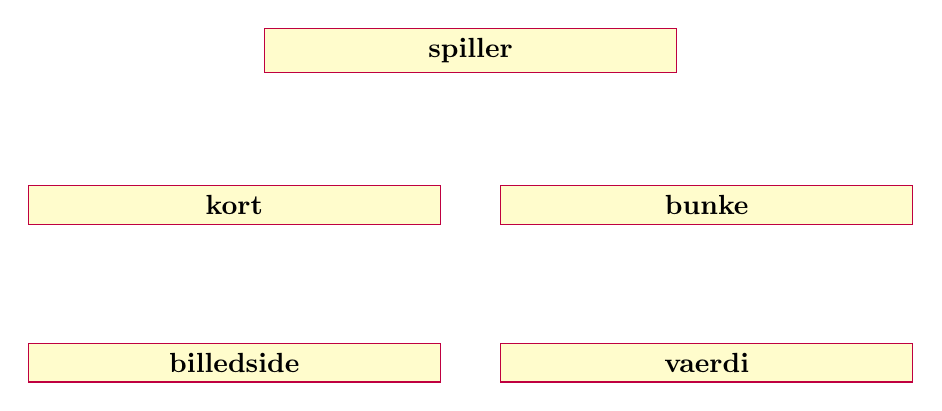
\begin{tikzpicture}
    \begin{class}[text width=5cm]{spiller}{0,0}
    \end{class}
    \begin{class}[text width=5cm]{kort}{-3,-2}
    \end{class}
    \begin{class}[text width=5cm]{bunke}{3,-2}
    \end{class}
    \begin{class}[text width=5cm]{billedside}{-3,-4}
    \end{class}
    \begin{class}[text width=5cm]{vaerdi}{3,-4}
    \end{class}
  \end{tikzpicture}
\end{center}
\vspace*{1cm}
\noindent Associationer:
\begin{center}
  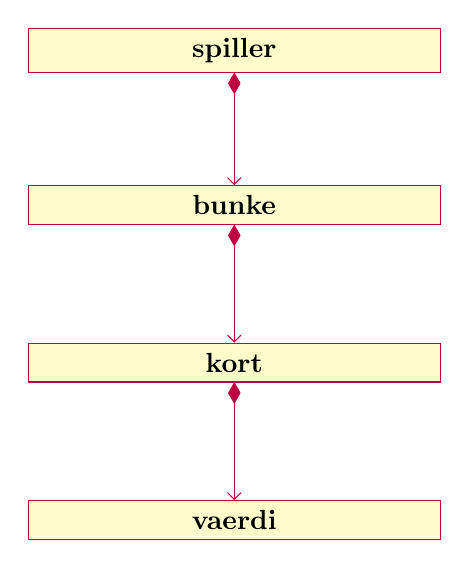
\begin{tikzpicture}
    \begin{class}[text width=5cm]{spiller}{0,0}
    \end{class}
    \begin{class}[text width=5cm]{bunke}{0,-2}
    \end{class}
    \begin{class}[text width=5cm]{kort}{0,-4}
    \end{class}
   \begin{class}[text width=5cm]{vaerdi}{0,-6}
    \end{class}
    \composition{spiller}{}{}{bunke}
    \composition{bunke}{}{}{kort}
    \composition{kort}{}{}{vaerdi}
  \end{tikzpicture}
\end{center}
\vspace*{1cm}
\noindent Properties:
\begin{center}
  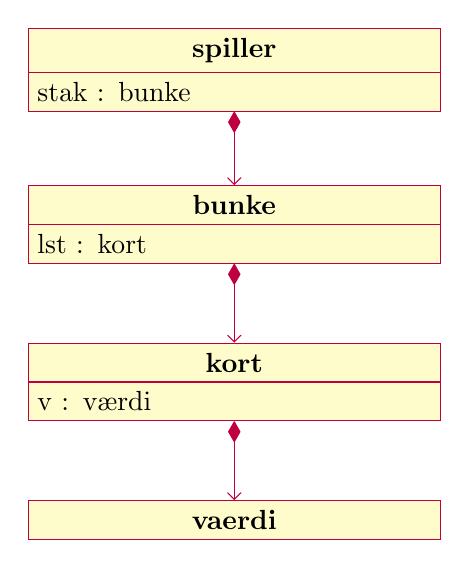
\begin{tikzpicture}
    \begin{class}[text width=5cm]{spiller}{0,0}
      \attribute{stak : bunke}
    \end{class}
    \begin{class}[text width=5cm]{bunke}{0,-2}
      \attribute{lst : kort}
    \end{class}
    \begin{class}[text width=5cm]{kort}{0,-4}
      \attribute{v : værdi}
    \end{class}
    \begin{class}[text width=5cm]{vaerdi}{0,-6}
    \end{class}
    \composition{spiller}{}{}{bunke}
    \composition{bunke}{}{}{kort}
    \composition{kort}{}{}{vaerdi}
  \end{tikzpicture}
\end{center}
\vspace*{1cm}
\noindent Methods:
\begin{center}
  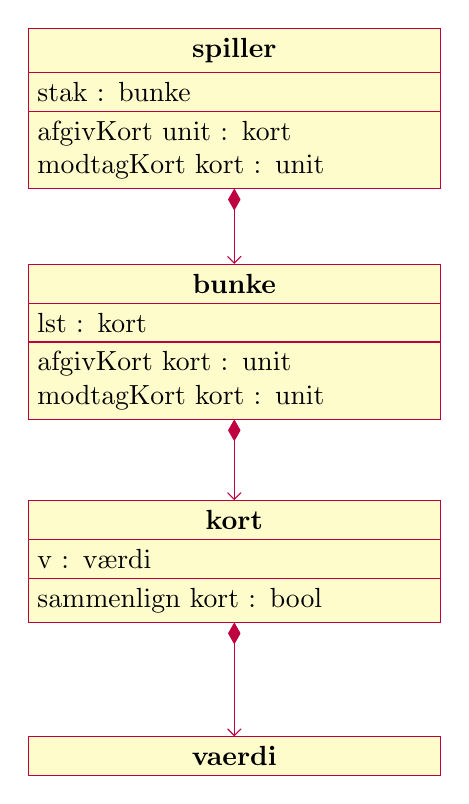
\begin{tikzpicture}
    \begin{class}[text width=5cm]{spiller}{0,0}
      \attribute{stak : bunke}
      \operation{afgivKort unit : kort}
      \operation{modtagKort kort : unit}
    \end{class}
    \begin{class}[text width=5cm]{bunke}{0,-3}
      \attribute{lst : kort}
      \operation{afgivKort kort : unit}
      \operation{modtagKort kort : unit}
    \end{class}
    \begin{class}[text width=5cm]{kort}{0,-6}
      \attribute{v : værdi}
      \operation{sammenlign kort : bool}
    \end{class}
    \begin{class}[text width=5cm]{vaerdi}{0,-9}
    \end{class}
    \composition{spiller}{}{}{bunke}
    \composition{bunke}{}{}{kort}
    \composition{kort}{}{}{vaerdi}
  \end{tikzpicture}
\end{center}

\noindent Correction:
\begin{center}
  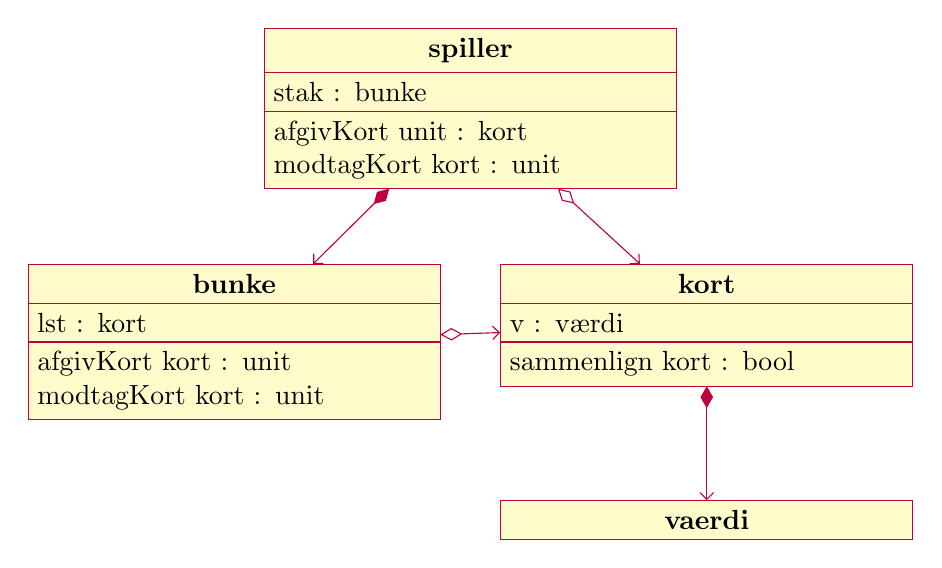
\begin{tikzpicture}
    \begin{class}[text width=5cm]{spiller}{0,0}
      \attribute{stak : bunke}
      \operation{afgivKort unit : kort}
      \operation{modtagKort kort : unit}
    \end{class}
    \begin{class}[text width=5cm]{bunke}{-3,-3}
      \attribute{lst : kort}
      \operation{afgivKort kort : unit}
      \operation{modtagKort kort : unit}
    \end{class}
    \begin{class}[text width=5cm]{kort}{3,-3}
      \attribute{v : værdi}
      \operation{sammenlign kort : bool}
    \end{class}
    \begin{class}[text width=5cm]{vaerdi}{3,-6}
    \end{class}
    \composition{spiller}{}{}{bunke}
    \aggregation{bunke}{}{}{kort}
    \composition{kort}{}{}{vaerdi}
    \aggregation{spiller}{}{}{kort};
  \end{tikzpicture}
\end{center}

\noindent Correction2:
\begin{center}
  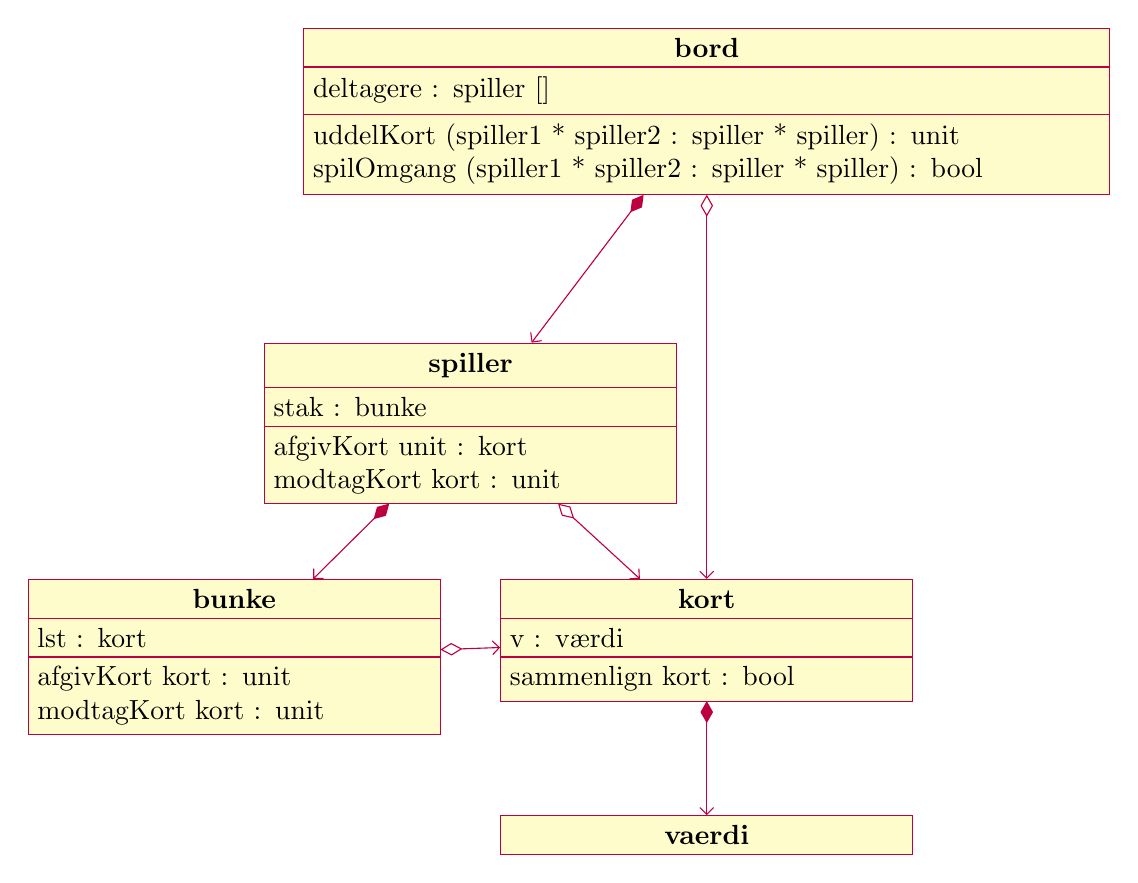
\begin{tikzpicture}
    \begin{class}[text width=10cm]{bord}{3,4}
      \attribute{deltagere : spiller []}
      \operation{uddelKort (spiller1 * spiller2 : spiller * spiller) : unit}
      \operation{spilOmgang (spiller1 * spiller2 : spiller * spiller) : bool}
    \end{class}
    \begin{class}[text width=5cm]{spiller}{0,0}
      \attribute{stak : bunke}
      \operation{afgivKort unit : kort}
      \operation{modtagKort kort : unit}
    \end{class}
    \begin{class}[text width=5cm]{bunke}{-3,-3}
      \attribute{lst : kort}
      \operation{afgivKort kort : unit}
      \operation{modtagKort kort : unit}
    \end{class}
    \begin{class}[text width=5cm]{kort}{3,-3}
      \attribute{v : værdi}
      \operation{sammenlign kort : bool}
    \end{class}
    \begin{class}[text width=5cm]{vaerdi}{3,-6}
    \end{class}
    \composition{bord}{}{}{spiller}
    \composition{spiller}{}{}{bunke}
    \aggregation{bunke}{}{}{kort}
    \composition{kort}{}{}{vaerdi}
    \aggregation{spiller}{}{}{kort}
    \aggregation{bord}{}{}{kort}
  \end{tikzpicture}
\end{center}

\end{document}
